%************************************************
\chapter{The MHM Cloud Infrastructure}\label{ch:our_cloud}
%************************************************

Now that we have the perfect communication channels, and before we dive into the development of the multi-platform application, let us take a look at the backend infrastructure that will run our Cloud Service.

We have a \textit{Ruby on Rails API} server set up as the backend for our application. This server is in charge of managing, collecting and updating the current Publications from the different clients of \textit{MHM} that use the eRecruiting application, and has a web front-end where we can manage the companies, add new ones and delete or edit the old ones.

We decided to let a separate server handle and organize the different Publications, because it saves us computing power and gives us a way to expand the apps content without having to publish a new version. Doing everything directly on the app, would require a lot of different connections and would take far longer than what's acceptable.

The server is also necessary for the remote search functionality and the management of certain functions that we will discuss on the upcoming chapters.

In order to keep all Publications up to date, the server connects every hour to all the registered Client eRecruiting Applications, one at a time, and collects information about the available Publications. This is accomplished through an \ac{XML} interface provided the eRecruiting System that collects all valid Publications and lists them as an \ac{XML} file.

The \ac{API} server then uses this \ac{XML} file to gather information about which Publications are new and which ones have been edited, so that it can perform actions on its database accordingly. The diagram in \autoref{fig:api} illustrates how this process works.

\begin{figure}[bth]
    \begin{center}
        {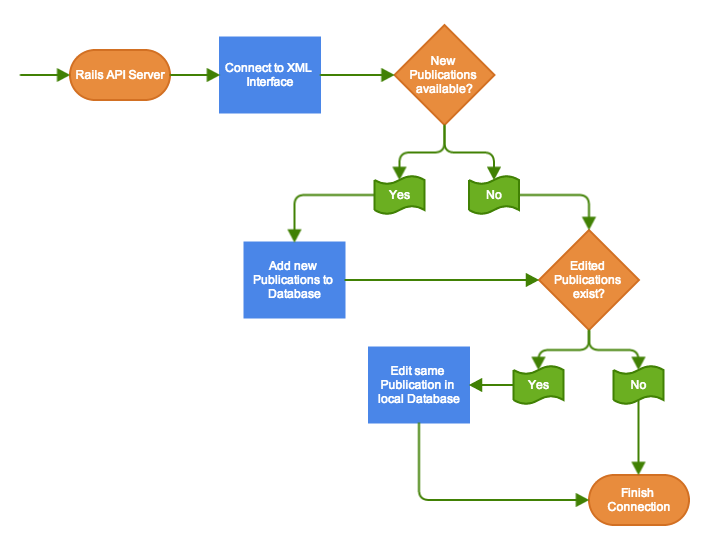
\includegraphics[width=1\linewidth]{gfx/api_flow}}
        \caption[Rails API Workflow]{Rails API Workflow}\label{fig:api}
    \end{center}
\end{figure}

Once the server is done updating the Publications, it is ready to accept incoming connections via its \ac{XML} and \ac{JSON} \ac{API}. The Rails Application exposes different methods for the different actions available to the mobile application. When one of this methods is called, the server performs a query with the database in order to find the matching Publications. It then builds an \ac{XML} or \ac{JSON} file containing all the returned Publications and sends it back to the calling agent.\\
\newline

The methods available to the mobile application are:
\begin{itemize}
\item Get available companies (\texttt{get\_companies})
\item Get the last 100 Job Publications (\texttt{get\_latest\_publications})
\item Send search parameters (\texttt{perform\_search})
\item Save unique device identifier (\texttt{save\_device\_token})
\item Save past searches (\texttt{save\_search})
\end{itemize}

The last two methods available are necessary for the implementation of push notifications. We will discuss this topic in further detail in \autoref{ch:building} and \autoref{ch:passive_com}.

Since almost all of the data management will be done inside the Rails Application, the mobile application doesn't need to keep track of old and new Publications. It can simply drop everything it has once the new data has been received and save this data to its local database, so that it i remains available, even if the user looses internet connectivity.

Now that we have an idea of how the \textit{MHM Cloud Backend} works and connects to the different eRecruiting Systems, let's dive right into the actual development of the MHM Job Portal Aggregator.




